\documentclass{article}
\usepackage[utf8]{inputenc}
\usepackage{textcomp}
\usepackage{gensymb}
\usepackage{geometry}
\usepackage{fancyhdr}
\usepackage{tkz-euclide}
\usepackage{ragged2e}
\usepackage{hyperref}
\usepackage{float}
\usepackage{tikz}
\usepackage{float}
\usepackage{multirow}
\usepackage{biblatex}
\usepackage[graphicx]{realboxes}
\addbibresource{refs.bib}

\pagestyle{fancy}
\geometry{top=3cm, bottom=2.5cm, left=3.5cm, right=3.5cm}
\rhead{CS-358}
\lhead{\leftmark}
\fancyfoot[R]{\leftmark}
\fancyfoot[C]{}
\fancyfoot[L]{Page \thepage}
\renewcommand{\footrulewidth}{1pt}
\usepackage{multicol}
\title{CS-358: Individual Project Proposal}
\author{Noa Ette - 363760\\Mateo Tiedra - 356525\\Kevan Lam - 356395\\Louis Larcher - 361002\\Ugo Novello - 329763\\Antoine Gautier - 356442}
\date{\today}

\begin{document}


\maketitle
\vspace{45mm}
\tableofcontents
\newpage
\section{Project Description: Autonomous 3d Object Scanner}

The core of this project idea is to make a mobile robot capable of identifying the object of interest and taking pictures of it from all (possible) angles. 
This would be paired with a desktop application that would receive the images and apply the user selected 3d reconstruction algorithm.\\


From this description we can identify several key components the project needs: \begin{enumerate}
    \item \texttt{The Robot}:
    \begin{description}
            \item[1.1] Navigate and plan routes around object.
            \item[1.2] Segment view and recognize object of interest.
            \item[1.3] Translate camera on z axis whilst tracking object of interest.
    \end{description}
    \item \texttt{The Desktop Application}:
    \begin{description}
        \item[2.1] User can choose object of interest.
        \item[2.2] Process images sent by robot using 3d reconstruction algorithms (NeRF \cite{mildenhall2020nerf}, 2DGS \cite{Huang2DGS2024}, Multi-view stereo)
    \end{description}
\end{enumerate}

Nowadays, one does not need specialised high end equipment in order to 3d scan objects. Most of us already have the sufficient equipment needed, a smartphone, given that it has a functioning camera and the adequate software. \\
For this project we will not be using a smartphone as it gives the robot higher usefulness and does not drastically increase complexity to have an integrated camera. 

In order to move the camera we will use an arm with two segments each powered by a stepper motor (like the Pixar lamp) fixed on top of the robot and oriented perpendicular to the wheels. In addition, the camera will be fixed to the arm using two servos offering roll and pitch control.


Most currently existing 3d Object scanners are catered to small objects \cite{desktop3dscanner}, rotating the object and photographing it from a fixed camera. We decided to take a different approach with the goal to give more flexibility while keeping the complexity as low as possible.


\newpage
\section{Related Projects}
We have looked at various related projects whilst trying to figure out how to design ours in the best possible manner.

We figured a mostly square base with two motors placed on diagonal wheels would be the most practical while being resource efficient and simple. This setup allows the "car" part of the robot to spin on itself, removing the need of having the arm holding the camera spin. This kind of movement is principally inspired by tanks, excavators and other tracked vehicles, except the two wheels on each side are independent instead of linked by a track.

The arm on the other hand takes inspiration from the many existing robotic or industrial arms existing. More particularly, we found this design \cite{cameraArm} which achieves a similar purpose as ours. Moving the motor for the second joint to the base is a key element of the design since it allows to have weaker motors and an overall lower center of gravity.

Unfortunately we have been unsuccessful in finding a project where a robot tracks an object, rotating around it. This poses a particular computer vision challenge as the robot needs to be able to recognise the object from completely distinct angles. Thanks to the fact that the robot will be navigating using video from an ESP32-CAM on the front of the robot, basic object tracking like those in opencv will most likely be sufficient.




\section{User Stories}

The final product of this project is something that could be useful to many people from different horizons. \\
In one case, one could imagine a real estate agent, wanting to provide virtual visits of a home he is selling. Instead of having to contact a freelance 3D artist to remodel the home, probably costing thousands, they would be able to simply 3d scan the area using the robot and software made in this project, saving plenty of time and money. Some companies have already ventured into real-estate specific 3d scanning \cite{matterport}. \\
Another imaginable use case is for professional 3d artists wanting to use realistic large objects in their 3d scenes. The conventional way to scan these objects would be to manually take pictures of them. Something that is very time consuming and sometimes requires particular gymnastics skills.
I personally have a little bit of experience with manually 3d scanning objects and can personally attest that, depending on the object, it can take a frustratingly long amount of time.

It could be an interesting demonstration for the EPFL Open House as it demonstrates the link between 3d art and computer science by leveraging an intelligent robot to optimise the workload of different career paths.

\section{Long term view}

Given a long term viewpoint, we could easily imagine different form factors being based on this project being developed for many different use cases. 

At a much larger scale, terrestrial and aerial 3d scanning robots could be used to map entire city's. Re-creating what would take thousands if not millions of man hours. This data could be used to train autonomous vehicles on real city's though simulation or for many other projects.

At a smaller scale, this technology could be redesigned on an aquatic form factor in order to map ocean floors and areas inaccessible by humans.

\newpage
\section{Physical description}

The robot takes the form of a square "car" with four wheels, 2 of which are powered by brushed motors. An ESP-32 cam on the front of the car allows to make decisions on the movement of the car regarding it environment, this will be further detailed in the next section. On top of the car lies an arm with two joints, each powered by a stepper motor. The arm is facing perpendicular to the direction of travel and on top of it is mounted a second esp-32 cam with an upgraded OV5640 camera. This camera contributes to the navigation but most importantly takes pictures of the object of interest from different angles and at different heights for later reconstruction. The camera is fixed to the arm using two servos, one controlling the pitch and the other the roll.

Regarding the control of all these motors, both esp-32 cam being quite limited in terms of I/O, we have a third micro-controller to handle them.

In terms of power, our thing will work on LiPo batteries, with a battery management board and voltage converters ensuring adequate power to all parts.

See images in the next page for a visual representation of the robot.

\newpage

\begin{figure}[H]
    \centering
    \begin{minipage}{0.45\textwidth}
        \centering
        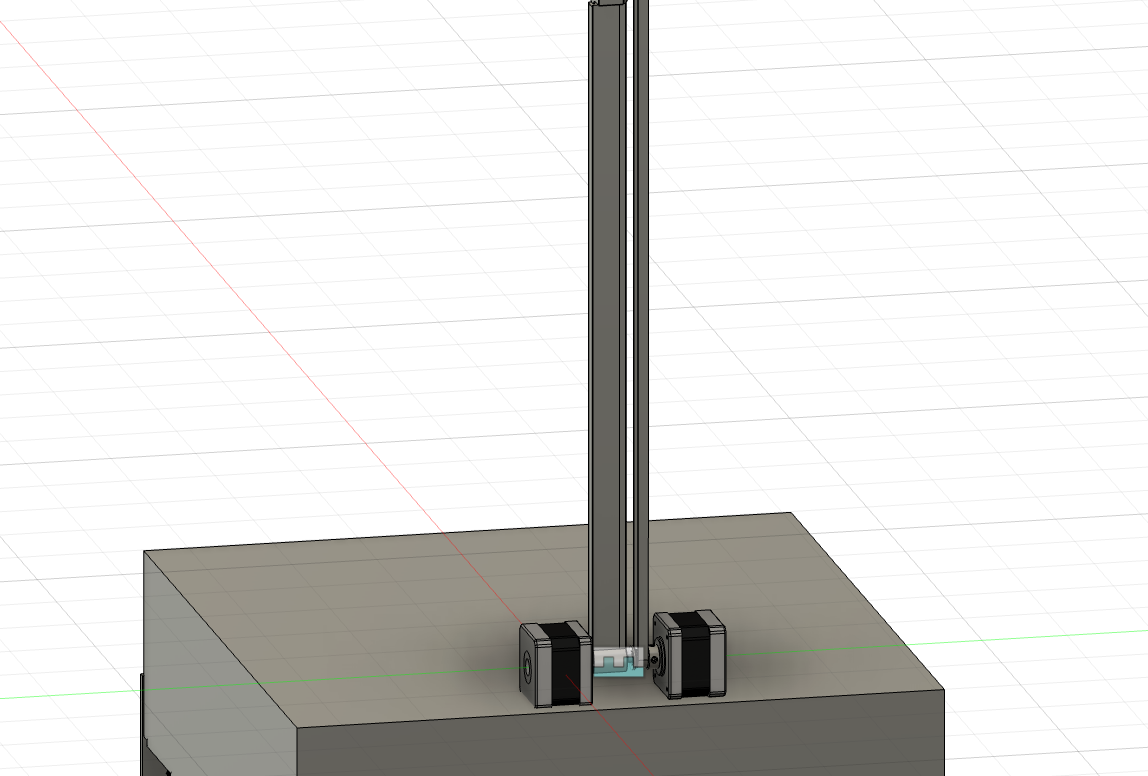
\includegraphics[width=\textwidth]{images/CAD-arm-with-stepper.png}
        \caption{Arm with stepper motors}
        \label{fig:image1}
    \end{minipage}
    \hfill
    \begin{minipage}{0.45\textwidth}
        \centering
        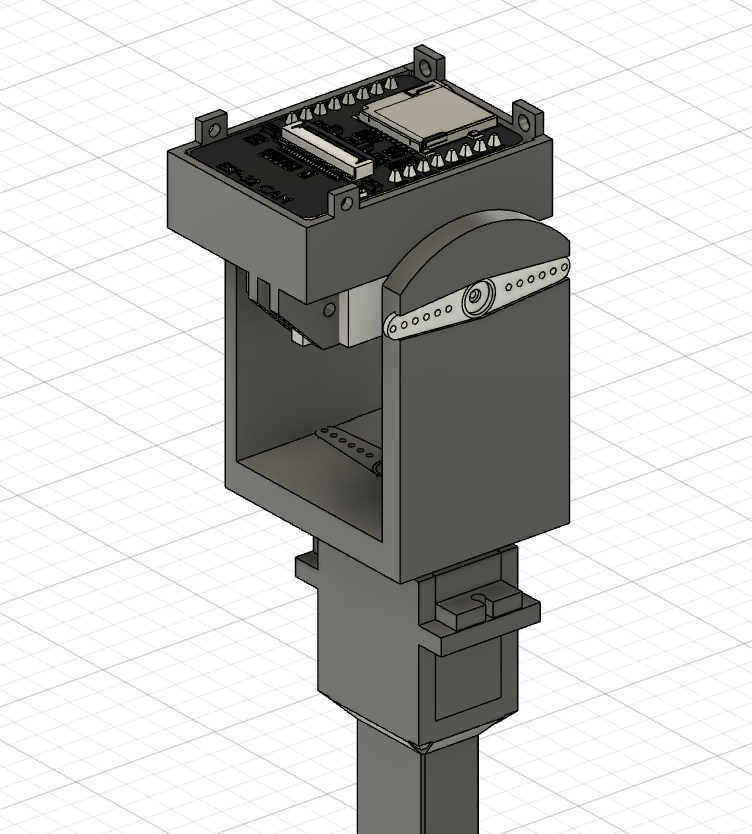
\includegraphics[width=\textwidth]{images/CAD-cam.png}
        \caption{Head of the arm with camera}
        \label{fig:image2}
    \end{minipage}
    \label{fig:sidebyside}
\end{figure}

\begin{figure}[H]
    \centering
    \begin{minipage}{0.45\textwidth}
        \centering
        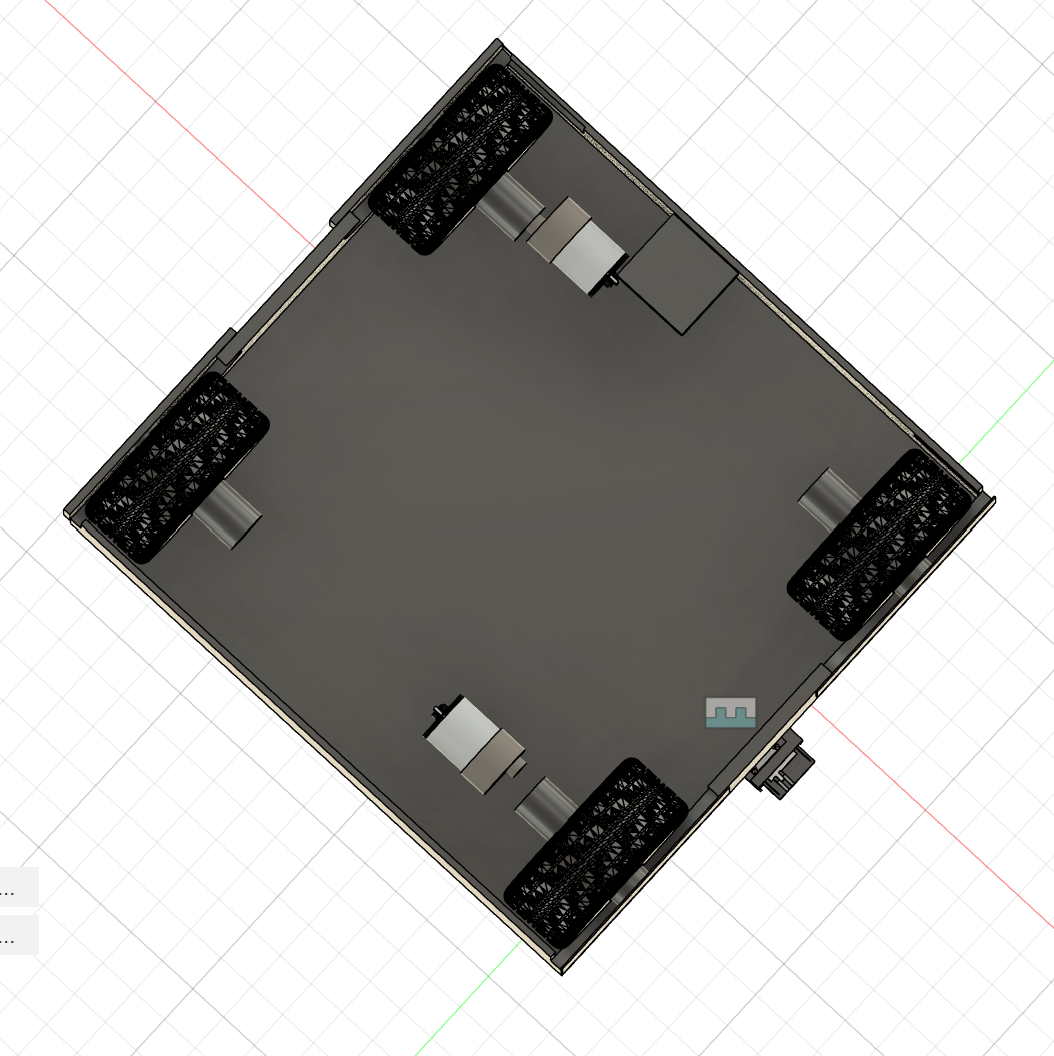
\includegraphics[width=\textwidth]{images/CAD-base-from-under.png}
        \caption{Base and wheels from underneath}
        \label{fig:image1}
    \end{minipage}
    \hfill
    \begin{minipage}{0.45\textwidth}
        \centering
        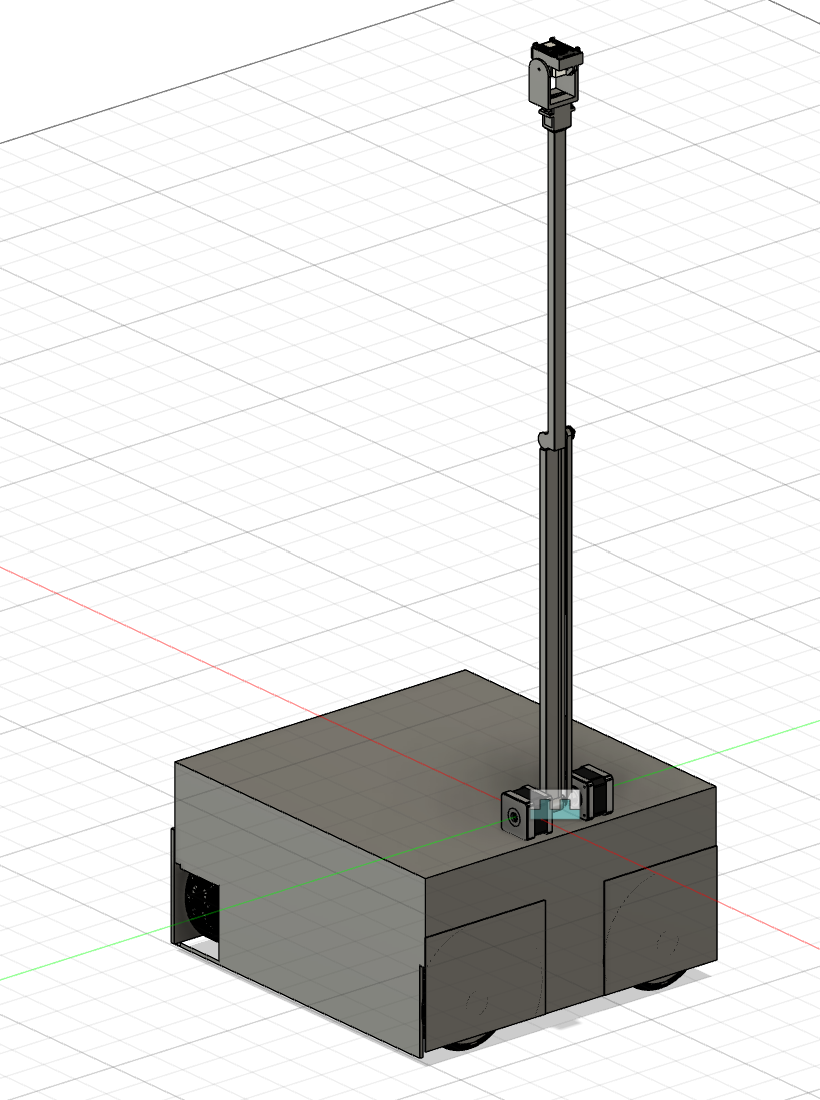
\includegraphics[width=\textwidth]{images/CAD-base-with.wheels.png}
        \caption{Full robot with wheels}
        \label{fig:image2}
    \end{minipage}
    \label{fig:sidebyside}
\end{figure}

\newpage

\section{Software description}

The Superscanner8000 software run on a computer connected to the robot through Wi-Fi. The program allows users to select an object within the camera’s field of view and adjust a parameter that specifies the level of precision needed, determining the number of photos the robot will capture. Once selected, the software guides the robot to navigate around the object, capturing images from various angles and distances. After gathering a sufficient number of images, the software processes them to generate a 3D model of the object, which can then be exported.

To enable the user to select an object for scanning, the software displays the live video feed from the robot camera on the screen, showing various objects in view. The user can click directly on the object of interest, which will then be detected and highlighted using Meta's open-source model, SAM 2.

\begin{figure}[H]
    \centering
    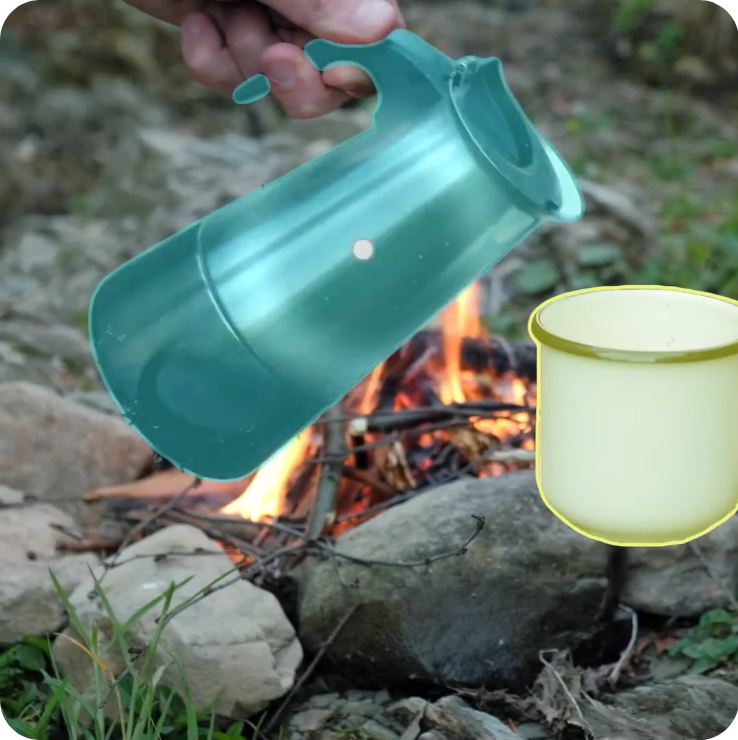
\includegraphics[width=0.5\linewidth]{images/sam2-example.png}
    \caption{Example of SAM 2's image segmentation}
    \label{fig:sam2-example}
\end{figure}

After the object is selected, the software directs the robot to move in a circular path around it. The robot moves in one direction while simultaneously using object segmentation to keep the object centered in the camera's field of view, rotating its entire body to maintain this alignment. Once it has completed a portion of the path, the software halts the robot, allowing it to capture images from different angles by adjusting the arm and raising or lowering the camera and the starts it again to move to the next position. This process is repeated until the robot has completed a full circle around the object. The user can stop the process at any time with a button on the software interface.

The images are transmitted from the robot to the computer in real time as the device moves and captures additional photos. Once the robot completes its data-gathering walk around the object and all images have been uploaded to the computer, the system initiates the 3D object conversion process using 3D reconstruction algorithms such as 2DGS \cite{Huang2DGS2024} and NeRF \cite{mildenhall2020nerf}.

\newpage
\section{Bill of materials}

\begin{center}
\Rotatebox{90}{%
\begin{tabular}{ ||c|c|c|c|c|c|| } 

\hline
Category & Type & Name & Site & Amount & Price \\
\hline
\hline
\multirow{4}{5em}{Actuators} 
& brushed motor & Chihai CHF-GM37-550ABHL & [In stock] & 2 & 25 \\ 
& brushed driver & L298N & [In stock] & 2 & 5\\
& stepper + driver & 17HS4401 + A4988 & [In stock] & 2 & 15 \\
& servo & SG90 & [In stock] & 2 & 3 \\
\hline
\hline
\multirow{4}{5em}{Controllers} 
& controller + camera & AIThinker esp32-cam & [In stock] & 2 & 4\\ 
& camera & OV5640 & \href{https://www.digikey.ch/fr/products/detail/seeed-technology-co-ltd/114993115/21277047}{digikey.ch} & 1 & 10.89\\ 
& microcontroller & ESP32-S2-DEVKITM-1U-N4R2 & \href{https://www.digikey.ch/fr/products/detail/espressif-systems/ESP32-S2-DEVKITM-1U-N4R2/16688756}{digikey.ch} & 1 & 7.27\\
& UART to USB & FTDI USB-to-serial & [In stock] & 1 & 2\\
\hline
\hline
\multirow{1}{5em}{Sensors}
& ultrasonic sensor & HC-SR04 & [In stock] & 1 & 2\\
\hline
\hline
\multirow{8}{5em}{Power}
& battery & Absima 11.1 V 6000 mAh 3S 50 C & \href{https://www.conrad.ch/fr/p/absima-pack-de-batterie-lipo-11-1-v-6000-mah-nombre-de-cellules-3-50-c-stick-xt90-3322657.html}{conrad.ch} & 1 & 51.95 \\
& BMS & 3S 12V 40A BMS & \href{https://www.elektronik-kaufen.ch/products/bms-3s-40a?variant=41643639701680&currency=CHF}{elektronik-kaufen.ch} & 1 & 5.5 \\
& heatsink & aluminum sheet & [In SPOT shop] & 1 & 10 \\
& battery plug male & XT90-S male plug & \href{https://www.conrad.ch/fr/p/reely-re-6702312-fiche-male-pour-batterie-xt90-s-dore-e-1-pc-s-2234104.html}{conrad.ch} & 2 & 1.9 \\
& battery plug female & XT90-S female plug & \href{https://www.conrad.ch/fr/p/reely-re-7471836-prise-femelle-pour-batterie-xt90-dore-e-1-pc-s-2490612.html}{conrad.ch} & 1 & 1.6 \\
& load balance plug & JST XH2.54 3p 20cm & \href{https://www.bastelgarage.ch/cable-de-connexion-jst-xh2-54-3p-20cm}{bastelgarage.ch} & 1 & 0.6 \\
& dc power plug & DC Socket Female Barrel Jack 5.5mm / 2.1mm & \href{https://www.bastelgarage.ch/dc-socket-female-barrel-jack-5-5mm-2-1mm-with-screw-terminals?search=dc%20female}{bastelgarage.ch} & 1 & 1.9\\
& voltage converter & LM2596 & [In stock] & 2 & 3 \\
\hline
\hline
\multicolumn{5}{|r|}{total cost} & 203.61\\
\hline
\hline
\end{tabular}
}%
\end{center}

\newpage

\section{Risk Assessment}

Here we will talk about potential risks for the success of the SuperScanner8000 project. Let’s start by focusing on the difficulties linked to the hardware. 

A basic concern is the voltage supply. We have decided to use a LIPO battery to supply our robot. This decision was made after making calculations and verifying that this battery would be enough for all our motors, drivers and microcontrollers. As shown in the bill of materials we also made sure to include all the extra components needed to accompany our LIPO battery. Of course, we will still have to make diagrams for all the electronics before plugging everything in to make sure it all works as planned.

Another typical concern is the power of our actuators. We have also run calculations for our wheels and our arm to make sure the brush/stepper motors were powerful enough. The servos for the camera should also be a good fit however we might have to adapt if we end up using a phone as our camera. All of this will of course have to be retested once we print out the pieces as shown in the GANTT chart.

Speaking of cameras, we also had a tough time finding the appropriate camera for this project. In the end we are choosing to go for the OV5640 camera which should have sufficient quality for recognition and reconstruction of 3d objects. We have thought of alternatives in case of this camera not working out for us, notably using a phone camera.

One last hardware concern is the stability of our SuperScanner8000. The arm should be able to move everywhere without throwing the robot out of balance. We have made multiple design choices like having the arm be orthogonal to the wheels or using a belt for the arm to attempt to reduce this problem however we will once again have to test this once we print the materials and assemble the robot.


Now moving onto the software side. 
One crucial concern is the one of communication between multiple microcontrollers. Our SuperScanner8000 will possess more than one microcontroller as the esp-32 driver does not have enough pins for all our motors. This means that we will have to make sure early on we can make our microcontrollers speak to each other. Notably here we want our camera to take a picture and then move around the object while also communicating to the other camera to make sure we don’t run into any obstacles. Thankfully all our microcontrollers are equipped with Wi-Fi which should let them communicate at a rapid speed.

This also leads us to our second concern which is the communication to the computer who is running the app. We will have to send photos taken by the cameras, compute our next move and send that information back. This will also have to be done through Wi-Fi and will have to be explored early on.

A very important problem we have to tackle in this project is the very basis of it : scanning 3d objects. Our team will have to code a program that is able to use the photos communicated by the robot to recognise and recreate accurate depictions of the 3d object. A lot of libraries and tools already exist for 3d scanning which will be of great help for us. We will also have to make sure we move around the object close enough so that we can recreate a good 3d model of high quality everywhere. This also means taking pictures of the underneath of a table for example which means we should be confident enough to guide our robot all around the 3d object. Optionally we also want to tackle the case of room scanning which involves the robot being capable of moving everywhere inside a room. It is possible we are being too optimistic about 3d scanning, that is why we have set some of the tasks as optional. This leaves us the freedom to spend more time on the basis of the project but also opens possibilities if we find time. Thankfully we have someone who knows a lot about 3d scanning : Noa Ette. He has already worked on such projects and feels confident that as a team we can succeed. With his guidance, the rest of the team should be able to learn more quickly about recognition and reconstruction basics.

Another closely linked problem is the obstacle avoidance issue. We will need this obstacle avoidance if we want to scan an object while others are around it or if we want to do the room scanning. Once again this is an optional task but it is important to state now what could potentially go wrong with it. The issue here will once again be to translate 2d images into something the SuperScanner8000 can understand and prepare against. Once again online libraries will be our biggest allies here and we will have to learn how to use them.

\newpage

\section{GANTT Chart}

\begin{figure}[H]
    \centering
    \rotatebox{90}{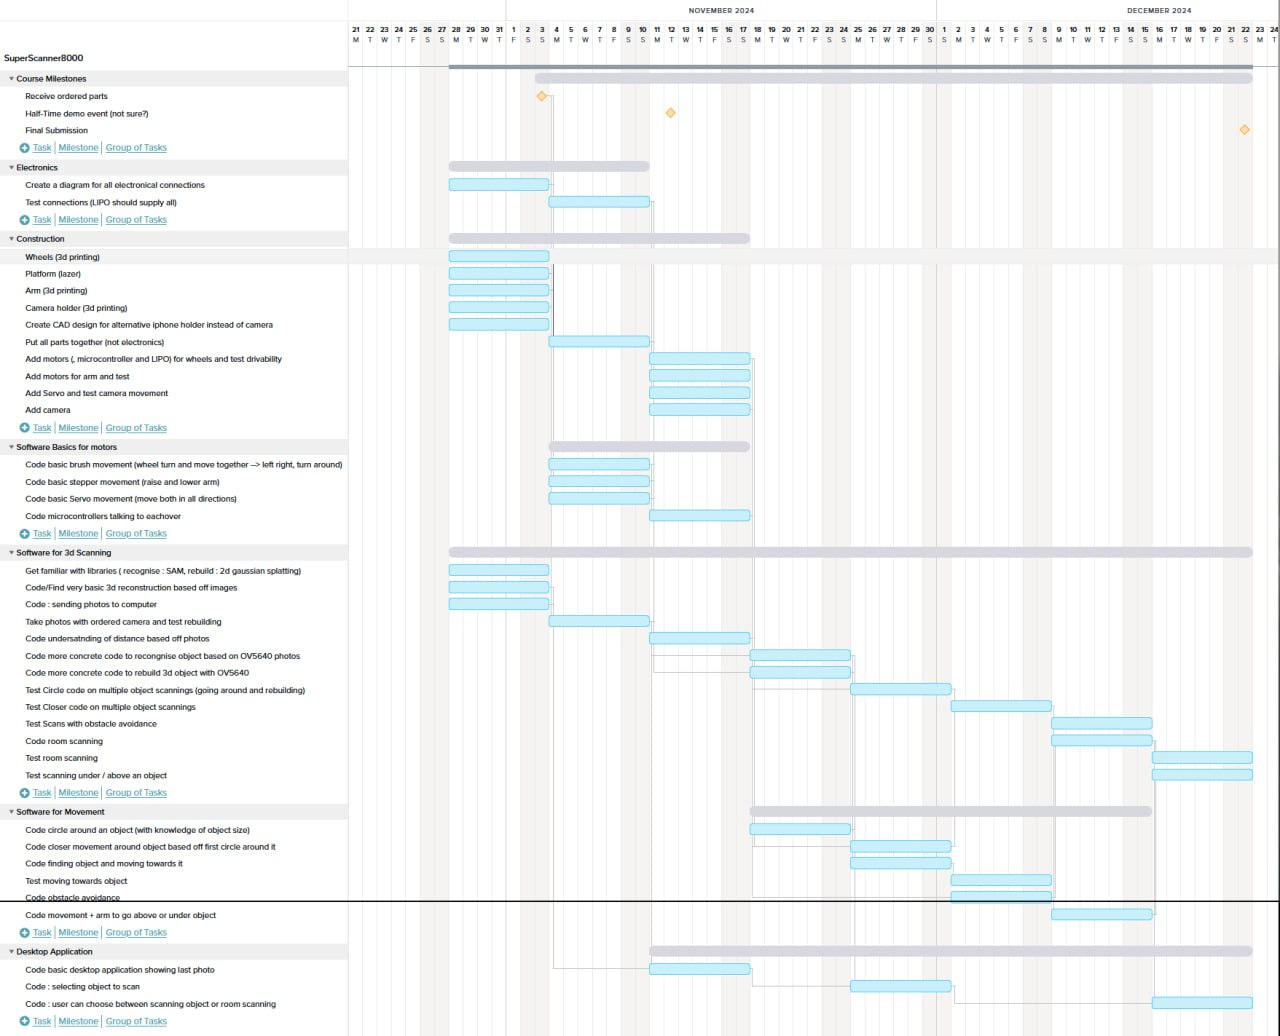
\includegraphics[width=1.3\linewidth]{images/gantt_chart.jpg}}
    \caption{Sceenshot of GANTT Chart made on teamgantt}
    \label{fig:gantt_chart}
\end{figure}

(Apologies for the bad quality, we couldn't export from teamgantt without using the pay option)

\newpage

\printbibliography

\end{document}
